\newfloat{equacao}{htpb}{equ}[chapter]
\floatname{equacao}{Equação}
\newcommand{\listequationsname}{Lista de equações}
\newcommand\crule[3][black]{\textcolor{#1}{\rule{#2}{#3}}}
\newcommand{\curso}[1]{\def\imprimircurso{#1}}
\newcommand{\palavraChaveUm}[1]{\def\imprimirpalavrachaveum{#1}}
\newcommand{\palavraChaveDois}[1]{\def\imprimirpalavrachavedois{#1}}
\newcommand{\cdu}[1]{\def\nomecdu{#1}}
\newcommand{\dataDaAprovacao}[1]{\def\imprimirdatadaaprovacao{#1}}
\newcommand{\membroConvidadoUm}[1]{\def\imprimirmembroconvidadoum{#1}}
\newcommand{\membroConvidadoDois}[1]{\def\imprimirmembroconvidadodois{#1}}
\newcommand\BackgroundPic{%
  \put(0,0){%
    \parbox[b][\paperheight]{\paperwidth}{%
      \vfill
      \centering
      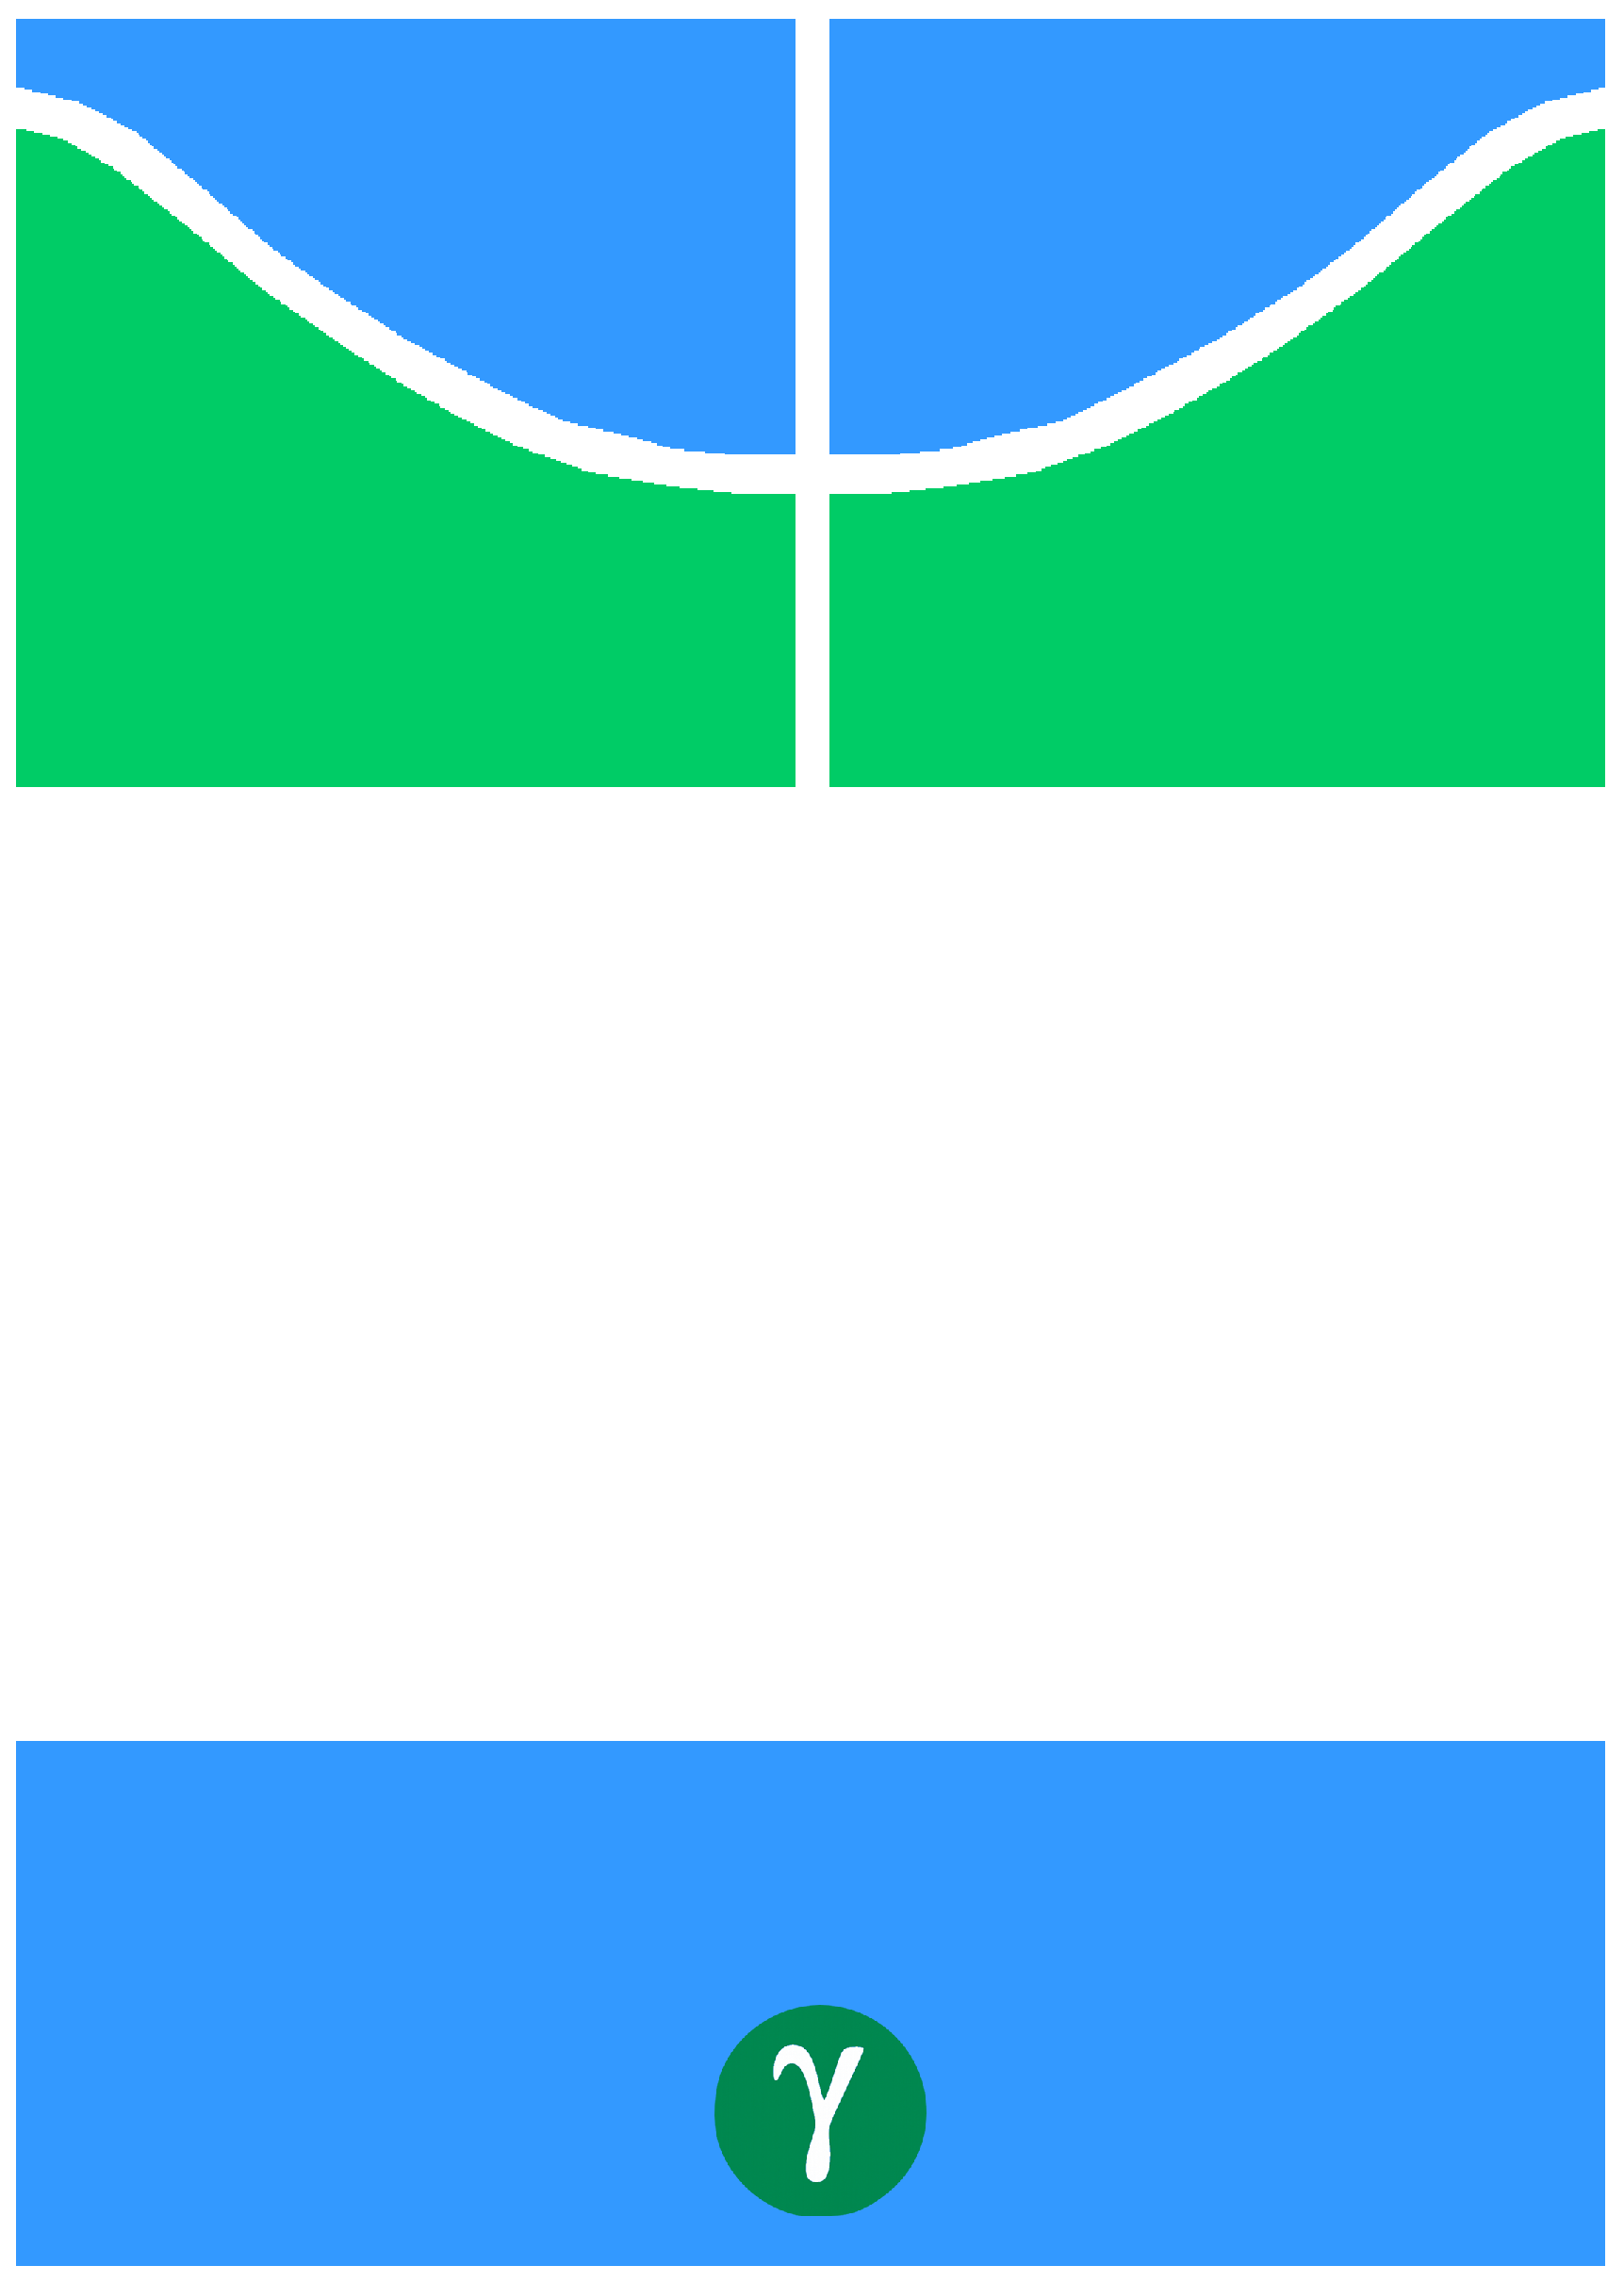
\includegraphics[width=\paperwidth,height=\paperheight,%
      keepaspectratio]{figuras/capa.eps}%
      \vfill
    }
  }
}
\renewcommand{\imprimircapa}{%
  \begin{capa}%
    \center
    \AddToShipoutPicture*{\BackgroundPic}
    \vspace*{2.2in}
    {\textbf{\center\large\imprimirinstituicao}}
    {\textbf{\center\large\imprimircurso}}
    \par
    \vspace{0.5in}
    {\ABNTEXchapterfont\bfseries\LARGE\imprimirtitulo}
    \vspace*{\fill}
    \begin{flushright}
      \textbf{{\large{Autor: \imprimirautor}}}
      \par
      \textbf{{\large{Orientador: \imprimirorientador}}}
    \end{flushright}
    \vspace*{0.2in}
    \textbf{{\large\imprimirlocal}}
    \textbf{{\center\large\imprimirdata}}
    \vspace*{2.2in}
  \end{capa}
}
